\section{Introducción}

\IEEEPARstart{L}{os} recientes avances tecnológicos y el amplio  uso de localización por sistemas de posicionamiento global (GPS),
identificación por radio frecuencia (RFID) y tecnologías en dispositivos móviles han hecho que las bases de datos
espacio temporales recolectadas hayan incrementado con un porcentaje acelerado. Esta gran cantidad de información
ha motivado a desarrollar eficientes técnicas, para procesar consultas acerca del comportamiento de los objetos en
movimiento, como descubrir patrones de comportamiento entre las trayectorias de objetos en un periodo continuo de tiempo. 

Los métodos que existen para consulta de trayectorias se centran principalmente en responder un único rango simple
de predicado  y consultas de vecinos mas cercanos   por ejemplo:  ``encontrar todos los objetos en movimiento que se
encontraban en la zona A a las 10 de la mañana (en el pasado)'' o ``encontrar el coche que condujo tan cerca como sea posible a
la ubicación B durante el intervalo de tiempo de 10 de la mañana a 1 de la tarde''.  Recientemente, diversos estudios se han centrado
en la consulta de los patrones para la captura del comportamiento de los objetos en movimiento reflejada en colaboraciones tales como
clusters móviles \cite{jensen2007continuous} \cite{kalnis2005discovering}, consulta de convoyes 
\cite{jeung2008discovery-1} y patrones de agrupación \cite{gudmundsson2006computing} \cite{benkert2008reporting}
\cite{vieira2009line}. Estos patrones descubren grupos de objetos en movimiento que tienen una ``fuerte'' relación en
el espacio durante un tiempo determinado. La diferencia entre todos esos patrones es la forma de definir 
la relación entre los objetos en movimiento y su duración en el tiempo. 

En este artículo se enfocará en el descubrimiento de patrones de agrupación, conocidos como ``flocks'', entre los objetos 
en movimiento de acuerdo
a las características de los objetos de estudio (animales, peatones, vehículos o fenómenos naturales), como 
interactúan entre si y como se mueven juntos \cite{laube2005finding} \cite{uno2005lcm}.  \cite{vieira2009line} 
define patrones de agrupamiento como el problema de identificar todos los grupos de trayectorias que permanecen
``juntas'' por la duración de un intervalo de tiempo dado. Consideramos que los objetos en movimiento están suficientemente
cerca si existe un disco con un
radio dado que cubre todos los objetos que se mueven en el patrón (Figura~\ref{fig:flockexample}). Una trayectoria satisface el 
patrón anterior, siempre y cuando suficientes trayectorias están contenidos dentro del disco para el intervalo de
tiempo especificado, es decir, la respuesta se basa no sólo en el comportamiento de una trayectoria dada, sino
también en los más cercanos a él. El enfoque actual para descubrir patrones de agrupación de movimiento consiste
en encontrar un conjunto adecuado de discos en cada instante de tiempo y luego la fusión de los resultados de un 
instante de tiempo a otro. Como consecuencia, el rendimiento y el número de patrones final depende del número
de los discos y cómo estos se combinan.

En el ejemplo de la Figura~\ref{fig:flockexample} se muestra un patrón de agrupamiento el cual contienen tres 
trayectorias {T1, T2, T3}
que están dentro de un disco en tres instantes de tiempo consecutivos. Los discos se pueden
mover libremente en el espacio bidimensional con el fin de acomodar los tres objetos en movimiento  y su centro no
tiene por que ser cualquiera de las localizaciones  de los objetos en movimiento. Esto hace que el
descubrimiento de agrupación de patrones sea mucho más complicada  porque hay un número infinito de posibles
colocaciones del disco en cualquier instante de tiempo y el posible número de combinaciones convierten
al problema en un problema NP-complejo.

La implementación de este algoritmo tiene diversas aplicaciones tales como: sistemas  integrados  de  transporte,
seguridad  y  monitoreo, seguimiento  a  grupos  de  animales  y  fenómenos  naturales,  encontrando  así  una
alternativa  diferente  para  solucionar  los  problemas  en  el  mundo,  analizando  como  se mueven  los  objetos
en  la  tierra  y  cuales  son  los  patrones  de  comportamiento  que existen entre si. 

En este artículo se muestra una comparación entre dos algoritmos, el propuesto por \cite{vieira2009line} y 
\cite{romero2011mining}, con el fin de identificar los problemas asociados a su rendimiento, y probando
estos algoritmos en distintos conjuntos de datos.


\begin{figure}
  \centering
  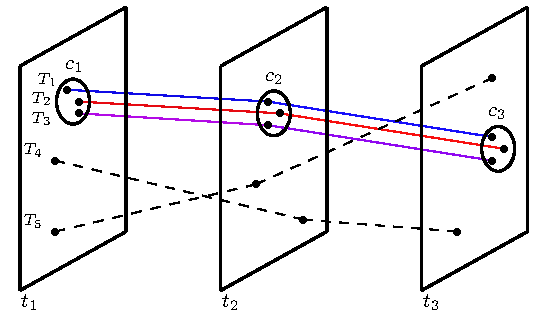
\includegraphics[scale=0.8]{pictures/flock_example}
  \caption{Ejemplo de patrones de agrupamiento} %(\cite{vieira2009line}).}
  \label{fig:flockexample}
\end{figure}